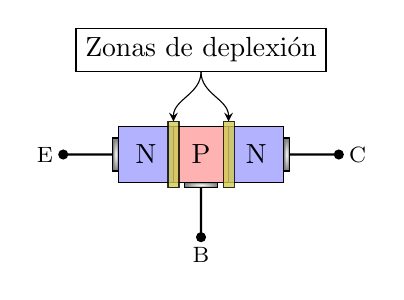
\begin{tikzpicture}[scale=0.7,>=stealth]
  \draw[fill=blue!30] (0,0) rectangle node{N} (1,1);
  \draw[fill=red!30] (1,0) rectangle node{P} (2,1);
  \draw[fill=blue!30] (2,0) rectangle node{N} (3,1);
  \filldraw[thick] (-0.1,0.5) -- (-1,0.5) circle (2pt) node[left, font=\footnotesize] {E};
  \filldraw[thick] (3.1,0.5) -- (4,0.5) circle (2pt) node[right, font=\footnotesize] {C};
  \filldraw[thick] (1.5,-0.1) -- (1.5,-1) circle (2pt) node[below, font=\footnotesize] {B};
  \shadedraw[color=black,fill=gray,inner color=white,outer color=gray] (-0.1,0.2) rectangle (0,0.8);
  \shadedraw[color=black,fill=gray,inner color=white,outer color=gray] (3,0.2) rectangle (3.1,0.8);
  \shadedraw[color=black,fill=gray,inner color=white,outer color=gray] (1.2,-0.1) rectangle (1.8,0);
  \draw[fill=yellow!60!gray,opacity=0.8] (0.9,-0.1) rectangle ++(.2,1.2);
  \draw[fill=yellow!60!gray,opacity=0.8] (1.9,-0.1) rectangle ++(.2,1.2);
  \node[draw, above] (T) at (1.5,2) {Zonas de deplexión};
  \draw[->] (T.south) to[out=270,in=90] (1,1.1);
  \draw[->] (T.south) to[out=270,in=90] (2,1.1);
\end{tikzpicture}
